\chapter*{Proposition 14}
\label{prop:14}

\begin{figure*}[ht]
    \begin{center}
    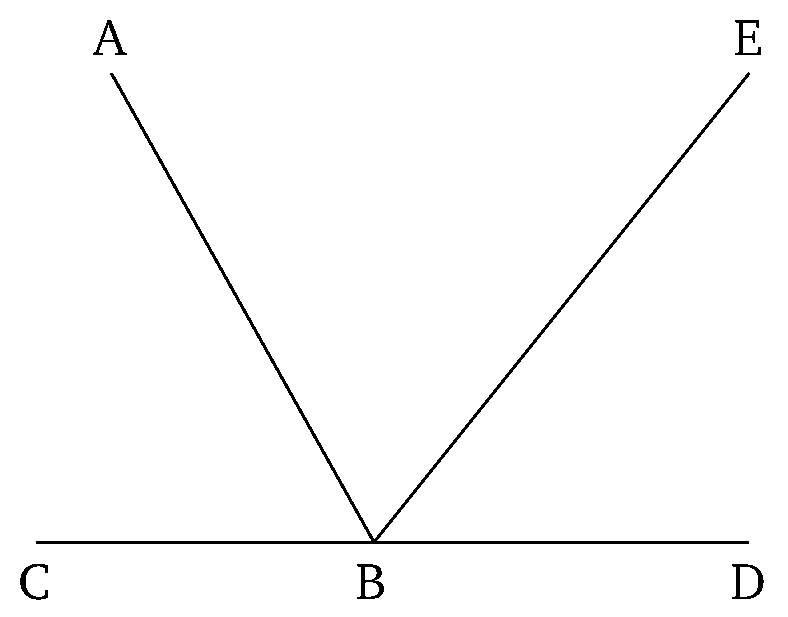
\includegraphics[width=0.5\linewidth]{figures/fig14e.eps}
    \label{fig:prop_14}
    \end{center}
\end{figure*}

If two straight-lines, not lying on the same side,  make adjacent angles (whose sum is) equal to two right-angles  with some straight-line, at a point on it, then the two straight-lines
will be straight-on (with respect) to one another.

For let two
straight-lines $BC$ and $BD$, not lying on the same side,  make adjacent angles $ABC$ and $ABD$ (whose sum is)
equal to two right-angles with some straight-line $AB$, at the point $B$ on it. I say
that $BD$ is  straight-on with respect to $CB$.

For if $BD$ is not straight-on to $BC$ then let $BE$ be straight-on to $CB$.

Therefore, since the straight-line $AB$ stands on the straight-line $CBE$, the (sum of the) angles $ABC$ and $ABE$ is thus equal to two right-angles [Prop.~1.13]. But (the sum of) $ABC$ and $ABD$ is also equal to two right-angles.
Thus, 
(the sum of angles) $CBA$ and $ABE$ is equal to (the sum of angles) $CBA$ and $ABD$ [C.N.~\ref{cn:1}]. Let (angle)
$CBA$ have been subtracted from both. Thus, the remainder $ABE$ is
equal to the remainder $ABD$ [C.N.~\ref{cn:3}], the lesser to the greater. The very thing is impossible. Thus, $BE$ is not straight-on with respect to $CB$. Similarly, we can
show that neither (is) any other (straight-line)   than $BD$.
Thus, $CB$ is straight-on with respect to $BD$.

Thus, if two straight-lines, not lying on the same side,  make adjacent angles (whose sum is) equal to two right-angles with some straight-line, at a point on it, then the two straight-lines
will be straight-on (with respect) to one another. (Which is) the very thing it
was required to show.


\section*{Commentary}

\begin{proposition}\label{proposition_14}\lean{Elements.Book1.proposition_14}\leanok
    $A$, $B$ are two distinct points on a line $AB$. $C$ and $D$ are two points on different sides of $AB$. $B$, $C$ are on a line $BC$. $B$, $D$ are on a line $BD$. $\angle~ABC + \angle~ABD$ is 180 degrees. Then, $BC$ and $BD$ must be the same line.
\end{proposition}
\begin{proof}
    \uses{proposition_13}\leanok
    Euclid only discussed the case where $E$ and $A$ are on the same side of $BD$, though the proof for other case is almost identical. 
\end{proof}
